\documentclass{article}
% ----------------------------------------------------------------------
% Define external packages, language, margins, fonts, new commands 
% and colors
% ----------------------------------------------------------------------
\usepackage[utf8]{inputenc} % Codification
\usepackage[english]{babel} % Writing idiom

\usepackage{pgfplots}
\pgfplotsset{compat=1.18}
\usepackage[T1]{fontenc}
\usepackage{imakeidx}
\usepackage{circuitikz}
\usetikzlibrary{positioning}
\usepackage[export]{adjustbox} % Align images
\usepackage{amsmath} % Extra commands for math mode
\usepackage{caption}
\usepackage{amssymb} % Mathematical symbols
\usepackage{anysize} % Personalize margins
    %\marginsize{2cm}{2cm}{2cm}{2cm} % {left}{right}{above}{below}
\usepackage{appendix} % Appendices
\usepackage{cancel} % Expression cancellation
\usepackage{placeins}
\usepackage{caption} % Captions
    \captionsetup{labelfont={bf}}
\usepackage{cite} % Citations, like [1 - 3]
\usepackage{color} % Text coloring
\usepackage{fancyhdr} % Head note and footnote
    \pagestyle{fancy}
    \fancyhf{}
    \fancyhead[L]{
        
\includegraphics[width=4cm]{Imagens/NovaFct.png}
    } % Left of Head note
    \fancyhead[R]{\footnotesize Controlo em Sistemas Ciber-físicos} % Right of Head note
    \fancyfoot[L]{\footnotesize MEEC} % Left of Footnote
    \fancyfoot[R]{\thepage  } % Center of Footnote
    %\fancyfoot[R]{\footnotesize Degree} % Right of Footnote
    \renewcommand{\footrulewidth}{0.4pt} % Footnote rule
\usepackage{float} % Utilization of [H] in figures
\usepackage{graphicx} % Figures in LaTeX
\usepackage[colorlinks = true, plainpages = true, linkcolor = istblue, urlcolor = istblue, citecolor = istblue, anchorcolor = istblue]{hyperref}
\usepackage{indentfirst} % First paragraph
\usepackage[super]{nth} % Superscripts
\usepackage{siunitx} % SI units

\usepackage{tocloft}%style the listofcontent to have dots
\renewcommand{\cftsecleader}{\cftdotfill{\cftdotsep}}

\usepackage[list=true, listformat=simple]{subcaption} % Subfigures

\usepackage{titlesec} % Font
    \titleformat{\section}{\Large\bfseries}{\thesection}{1em}{}
    \titleformat{\subsection}{\large\bfseries}{\thesubsection}{1em}{}
    \titleformat{\subsubsection}{\normalsize\bfseries}{\thesubsubsection}{1em}{}
    %\fancyfoot[C]{\thepage}

%code
\usepackage[breakable]{tcolorbox}

\graphicspath{ {Imagens/.} }

% Code highlighting
\usepackage{listings}
\lstset{ 
    language=Matlab,
    frame=single,
    numbers=left,
    numberstyle=\tiny,
    stepnumber=1,
    numbersep=5pt,
    backgroundcolor=\color{cellbackground}, % background color for the code block
    keywordstyle=\color{blue}\bfseries,
    commentstyle=\color{dkgreen},
    stringstyle=\color{red},
    breaklines=true,
    breakatwhitespace=false,
    showspaces=false,
    showstringspaces=false,
    showtabs=false,
    captionpos=b,
}

%pseudocode styling
\newcounter{nalg}[section] % defines algorithm counter for chapter-level
\DeclareCaptionLabelFormat{simple}{Algoritmo \thenalg} % defines a new caption label as Algorithm x.y
\lstnewenvironment{algorithm}[1][] % defines the algorithm listing environment
{
    \vspace{1ex}
    \crefstepcounter{nalg} % increments algorithm number
    \captionsetup{labelformat=simple,labelsep=colon,position=top} % set caption position to top
    \lstset{ % this is the style
        mathescape=true,
        frame=tB,
        numbers=left, 
        numberstyle=\tiny,
        basicstyle=\scriptsize, 
        keywordstyle=\color{black}\bfseries\em,
        keywords={input, output, return, datatype, function, in, if, else, foreach, while, begin, end}, % add the keywords you want, or load a language as Rubens explains in his comment above.
        numbers=left,
        xleftmargin=.04\textwidth,
        #1 % this is to add specific settings to an usage of this environment (for instance, the caption and referable label)
    }
}
{}

% Exact colors from NB
\definecolor{incolor}{HTML}{303F9F}
\definecolor{outcolor}{HTML}{D84315}
\definecolor{cellborder}{HTML}{CFCFCF}
\definecolor{cellbackground}{HTML}{F7F7F7}
\definecolor{commentcolour}{rgb}{0.42, 0.45, 0.51}
\definecolor{string}{rgb}{0.42, 0.45, 0.51}

\usetikzlibrary{shapes,arrows}
\tikzstyle{block} = [draw, rectangle, 
    minimum height=2.5em, minimum width=3.5em]
\tikzstyle{sum} = [draw, circle, node distance=1cm]
\tikzstyle{input} = [coordinate]
\tikzstyle{output} = [coordinate]
\tikzstyle{pinstyle} = [pin edge={to-,thin,black}]


% Random text (not needed)
\usepackage{lipsum}
\usepackage{duckuments}

% New and re-newcommands
\newcommand{\sen}{\operatorname{\sen}} % Sine function definition
\newcommand{\HRule}{\rule{\linewidth}{0.5mm}} % Specific rule definition
\renewcommand{\appendixpagename}{\LARGE Appendices}

% Colors
\definecolor{istblue}{RGB}{28, 118, 196}
\definecolor{dkgreen}{rgb}{0,0.6,0}

	
\usepackage{cleveref}
\usepackage{eurosym} %for euros

\usepackage{glossaries}

% -------------------------
% Glossary Entries
% -------------------------
\makeglossaries
\newglossaryentry{phi}{
    name= {$\varphi$},
    description={Orientation (heading) angle of the tractor}
}

\newglossaryentry{omega}{
    name={$\omega$},
    description={Angular velocity (steering input) of the tractor}
}

\newglossaryentry{length}{
    name=\ensuremath{l},
    description={Distance between the tractor and the trailer pivot point}
}

\newglossaryentry{valveOpening}{
    name=\ensuremath{z},
    description={Opening of the sprayer valve; $z \in [0,1]$}
}

\newglossaryentry{lyapunov}{
    name={$V(x,\zeta)$},
    description={Control Lyapunov Function used for guaranteeing stability}
}

\newglossaryentry{x_dot}{
    name=\ensuremath{\dot{x}},
    description={Variation in x}
}

\newglossaryentry{y_dot}{
    name=\ensuremath{\dot{y}},
    description={Variation in y}
}

\newglossaryentry{varphi_dot}{
    name=\ensuremath{\dot{\varphi}},
    description={Variation in the angle of the tractor}
}

\newglossaryentry{theta_dot}{
    name=\ensuremath{\dot{\theta}},
    description={Variation in the angle of the trailer}
}

\newacronym{clf}{CLF}{Control Lyapunov Function}

%%%%%%%%%%%%%%%%%%%%%%%%%%%%%%%%%%%%%%%%%%%%%%%%%%%%%%%%%%%%%%%%%%%%%%%%
%                                 Document                             %
%%%%%%%%%%%%%%%%%%%%%%%%%%%%%%%%%%%%%%%%%%%%%%%%%%%%%%%%%%%%%%%%%%%%%%%%
\begin{document}

% ----------------------------------------------------------------------
% Cover
% ----------------------------------------------------------------------
\begin{center}
    \begin{figure}
        \vspace{-1.0cm}
        
\includegraphics[scale = 1, left]{Imagens/NovaFct.png} % Nova logo
    \end{figure}

    \mbox{}\\[2.0cm]
    \textsc{\Huge Mestrado em Engenharia Eletrotécnica e de Computadores}\\[2.5cm]
    \textsc{\LARGE Controlo em Sistemas Ciber-físicos}\\[2.0cm]
    \HRule\\[0.4cm]
    {\large \bf { 
        Automation Control for a Tractor used for spraying trees\\
    }[\texttt{EN}]}\\[0.2cm]
    \HRule\\[1.5cm]
\end{center}

\begin{flushleft}
    \textbf{Authors:}
\end{flushleft}

\begin{center}
    António Canteiro\\
    Filipe Cavalheiro\\
    Rafael Louro
\end{center}

    \vspace{4cm}

    \begin{center}
        \large \bf 2025/2026 -- 1º Semestre
    \end{center}

    \thispagestyle{empty}

    \setcounter{page}{0}

    \newpage

    \newpage

    \renewcommand{\contentsname}{Table of contents}
    \tableofcontents % Generates the table of contents
    \newpage

    \renewcommand{\listfigurename}{List of Images}
    \listoffigures
    \newpage

    \printglossary
    \newpage

    \section{Objectives of the Project}

    Given the prevalence of olive oil production in Portugal and Spain, there is a need to automate some of the processes associated to this activity. One of these processes is the spraying of product upon the rows of olive trees, accomplished by driving a tractor towing the spraying trailer.
    This project aims to automate the driving of the tractor while reducing operational costs.\\

    \begin{figure}[H]
        \centering
        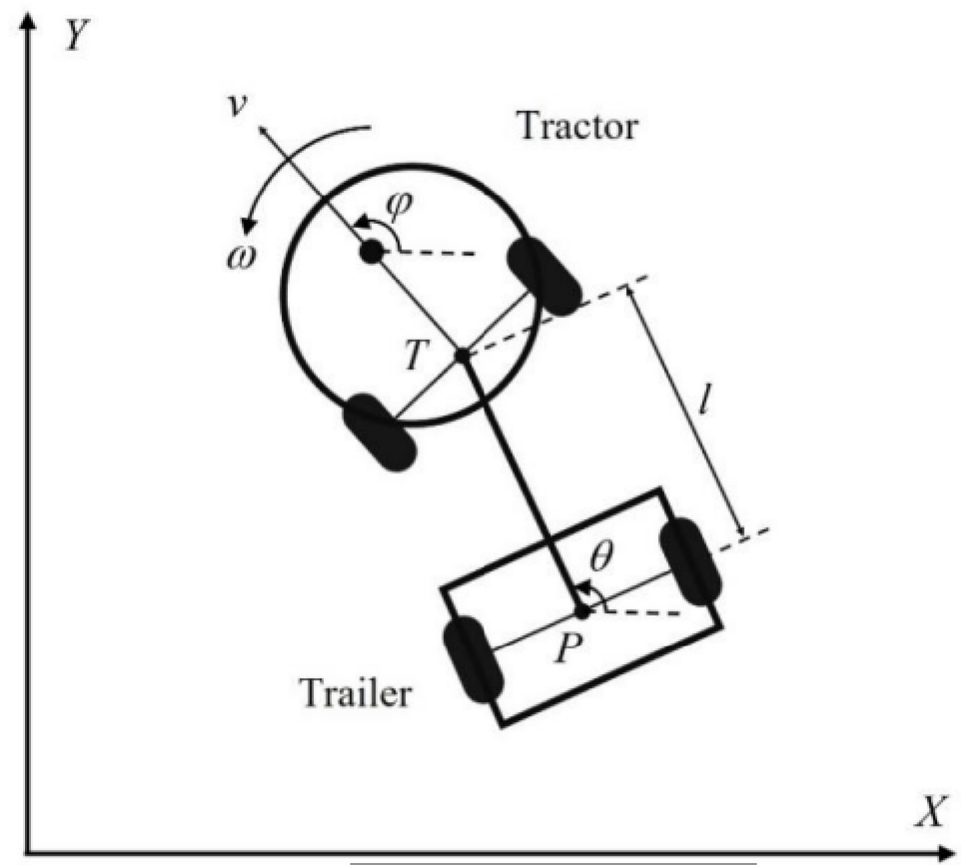
\includegraphics[width=0.5\textwidth]{Imagens/tractor.png} 
        \caption{Tractor model}
        \label{fig:tractor}
    \end{figure}

    The dynamical model of the point P is given by:

    \begin{equation}
        \begin{aligned}
            &\gls{x_dot} = v \cos(\varphi - \theta)\cos(\theta) \\
            &\gls{y_dot} = v \cos(\varphi - \theta)\sin(\theta) \\
            &\gls{varphi_dot} = \omega \\
            &\gls{theta_dot} = \frac{v}{l} \sin(\varphi - \theta)
        \end{aligned}
        \label{eq:trailer}
    \end{equation}

    The proposed solutions is split into three tasks of rising complexity.\\
    
    The \textbf{first task} is to design a controller that should be able to drive the tractor to the reference \( [10 \ 10]^{\top} \). The controller function will receive a value for the current state and output the actuation.\\

    The \textbf{second task} is to design a controller that enables the tractor to follow straight lines along the orchard, even in the presence of terrain disturbances such as irregularities or small variations in velocity. The controller receives as inputs the full state of the tractor ($x, y, \phi, \theta$) and the desired velocity along the line. The expected behavior is for the tractor to maintain its lateral position near $x = 0$ while moving along $y$ at the specified speed, ensuring precise alignment and minimal lateral deviation.\\

    The \textbf{third task} is to design a complete controller for the tractor to perform autonomous spraying operations in the orchard. The controller must optimize the cost per hectare while satisfying all constraints, including tank capacity, spraying range, and tree avoidance. The goal is to deliver 8 ml of product per tree, assuming that any application within a 4-meter radius around the trunk counts as valid. If the tractor or the sprayer collides with any tree, a penalty cost of \geneuro 1000 is incurred.\\

   Because the test environment changes for each task, the corresponding environment description, results, and task-specific considerations are presented together with each task. The controller, however, is identical across all tasks; therefore, it is described here in full to avoid repetition.

    The structure of the controller is based on a \gls{clf}, obtained by solving the following optimization problem:
    \begin{align*}
        \underset{u}{\text{min}} &\quad \|u\|^2 \\
        \text{s.t.} \quad & \dot{V}(x,\zeta) \leq -\alpha V(x,\zeta), \\
        & u \in U,
    \end{align*}
    where \gls{lyapunov} is a quadratic Lyapunov function. For practicality, the model used for controller design is that of the tractor alone; the trailer is expected to follow its trajectory. Even with this simplification, the model has relative degree greater than one, requiring the use of backstepping. The tractor model therefore takes the form
    \begin{align*}
        \dot{x} &= g_0(\zeta), \\
        \dot{\zeta} &= g_1(\zeta,u),
    \end{align*}
    where $x = [x\;\; y]^T$ are the positional states of the tractor, $\zeta = \varphi$ is its heading, and
    \begin{align*}
        g_0(\varphi) &=
        \begin{bmatrix}
            v \cos(\varphi) \\
            v \sin(\varphi)
        \end{bmatrix}, 
        &
        g_1(\varphi,u) &= u.
    \end{align*}

    The derivatives of these functions ($\dot{g}_1 = 0$) are given by
    \begin{align*}
        \dot{g}_0(\varphi) &=
        \begin{bmatrix}
            -v \dot{\varphi} \sin(\varphi) \\
            v \dot{\varphi} \cos(\varphi)
        \end{bmatrix}
        =
        u \cdot
        \begin{bmatrix}
            -v \sin(\varphi) \\
            v \cos(\varphi)
        \end{bmatrix}
        = u \cdot \dot{g}_{0,u}(\zeta).
    \end{align*}

    A partial controller is designed for $\dot{x}$ such that $x$ is driven toward a given reference:
    \begin{equation*}
        \kappa_0(x) = -\beta(x - \text{ref}),
    \end{equation*}
    with derivative
    \begin{align*}
        \dot{\kappa}_0(x) &= -\beta \dot{x}, \\
        \Leftrightarrow\quad
        \dot{\kappa}_0(\zeta) &= -\beta g_0(\zeta),
    \end{align*}
    where $\text{ref}$ is the reference position and $\beta$ is a tuning gain.

    We define the partial tracking error as
    \begin{align*}
        e &= \dot{x} - \kappa_0(x)
        = g_0(\zeta) - \kappa_0(x).
    \end{align*}

    The partial Lyapunov function is then
    \begin{align*}
        V_0(x,\zeta) &= \tfrac{1}{2} \|\dot{x} - \kappa_0(x)\|^2, \\
        \dot{V}_0(x,\zeta) &= (g_0(\zeta) - \kappa_0(x))^T \dot{g}_0(\zeta).
    \end{align*}

    The full Lyapunov function and its derivative are
    \begin{align*}
        V(x,\zeta,e) &= V_0(x,\zeta) + \tfrac{1}{2}\|e\|^2, \\
        \dot{V}(x,\zeta,e) &= \dot{V}_0(x,\zeta) + e^T \dot{e} \\
        &= \dot{V}_0(x,\zeta) 
        + (g_0(\zeta) - \kappa_0(x))^T 
        \left( u \cdot \dot{g}_{0,u}(\zeta) - \dot{\kappa}_0(\zeta) \right).
    \end{align*}

    To obtain the full controller $\kappa(x)$, we compute the stationary point of the Hamiltonian:
    \begin{equation*}
        H(u,\lambda) = \tfrac{1}{2}\|u\|^2 + \lambda(\dot{V} + \alpha V).
    \end{equation*}

    Solving for $u$ yields the control law:
    \begin{equation*}
        \kappa(x,\zeta,e)
        = -\frac{e^T \dot{\kappa}_0(\zeta) + \dot{V}_0(x,\zeta) + \alpha V(x,\zeta,e)}
        {e^T \dot{g}_{0,u}(\zeta)}.
    \end{equation*}

    This controller is applied only when the following feasibility conditions are satisfied:
    \begin{equation*}
        e^T \dot{\kappa}_0(\zeta) + \dot{V}_0(x,\zeta) + \alpha V(x,\zeta,e) \ge 0,
        \qquad
        \|e^T \dot{g}_{0,u}(\zeta)\|^2 \neq 0.
    \end{equation*}

    \section{Proposed Solutions}
    \subsection{First Task}
    
    \indent In the first part we drive the tractor to the reference. \( [10 \ 10]^{\top} \). Simply by passing to the \gls{clf} the reference as we can see~\cref{fig:ex1_results} it follows it with out any kind of problem.

    \begin{figure}[H]
        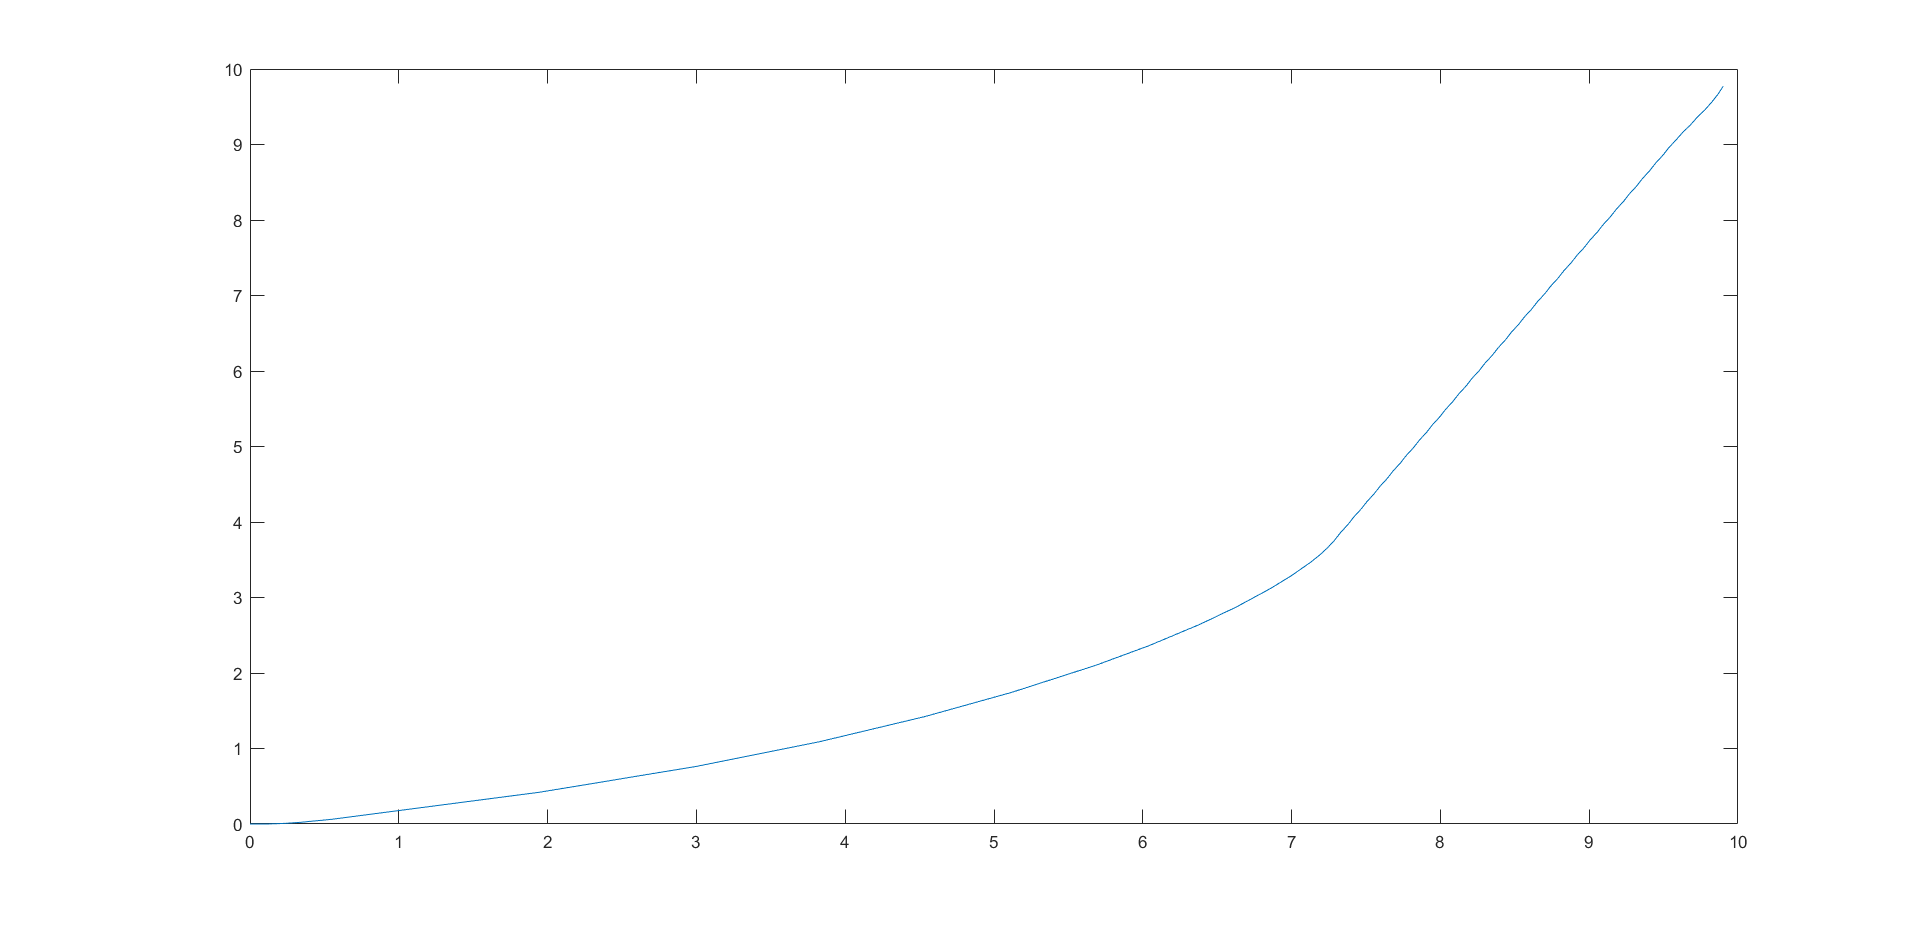
\includegraphics[width=\linewidth]{Imagens/ex1_results.png}
        \caption{Path in x,y of the tractor}
        \label{fig:ex1_results}
    \end{figure}
        
    \subsection{Second Task}~\label{sec:second_task}

    The objective of the second part of the project is to ensure safe navigation of the tractor by considering its dynamic model, external disturbances, and implementing a stable control strategy. In this task, the tractor must follow a line of trees while maintaining a safe distance to avoid collisions, as each collision results in a 1000 \geneuro penalty. 

    The main difference compared to the previous task is that the reference trajectory is now defined as a sequence of discrete points, one per tree, being the trees spaces with 4 m between each one. Once the tractor reaches a distance of \SI{0.2}{\meter} from the current reference point, the controller updates the reference to the next tree in the row. Since the controller is a \gls{clf} and therefore exponentially stable, maintaining safe clearance from the trees was achieved by simply tracking these sequential reference points.

    \begin{figure}[H]
        \centering
        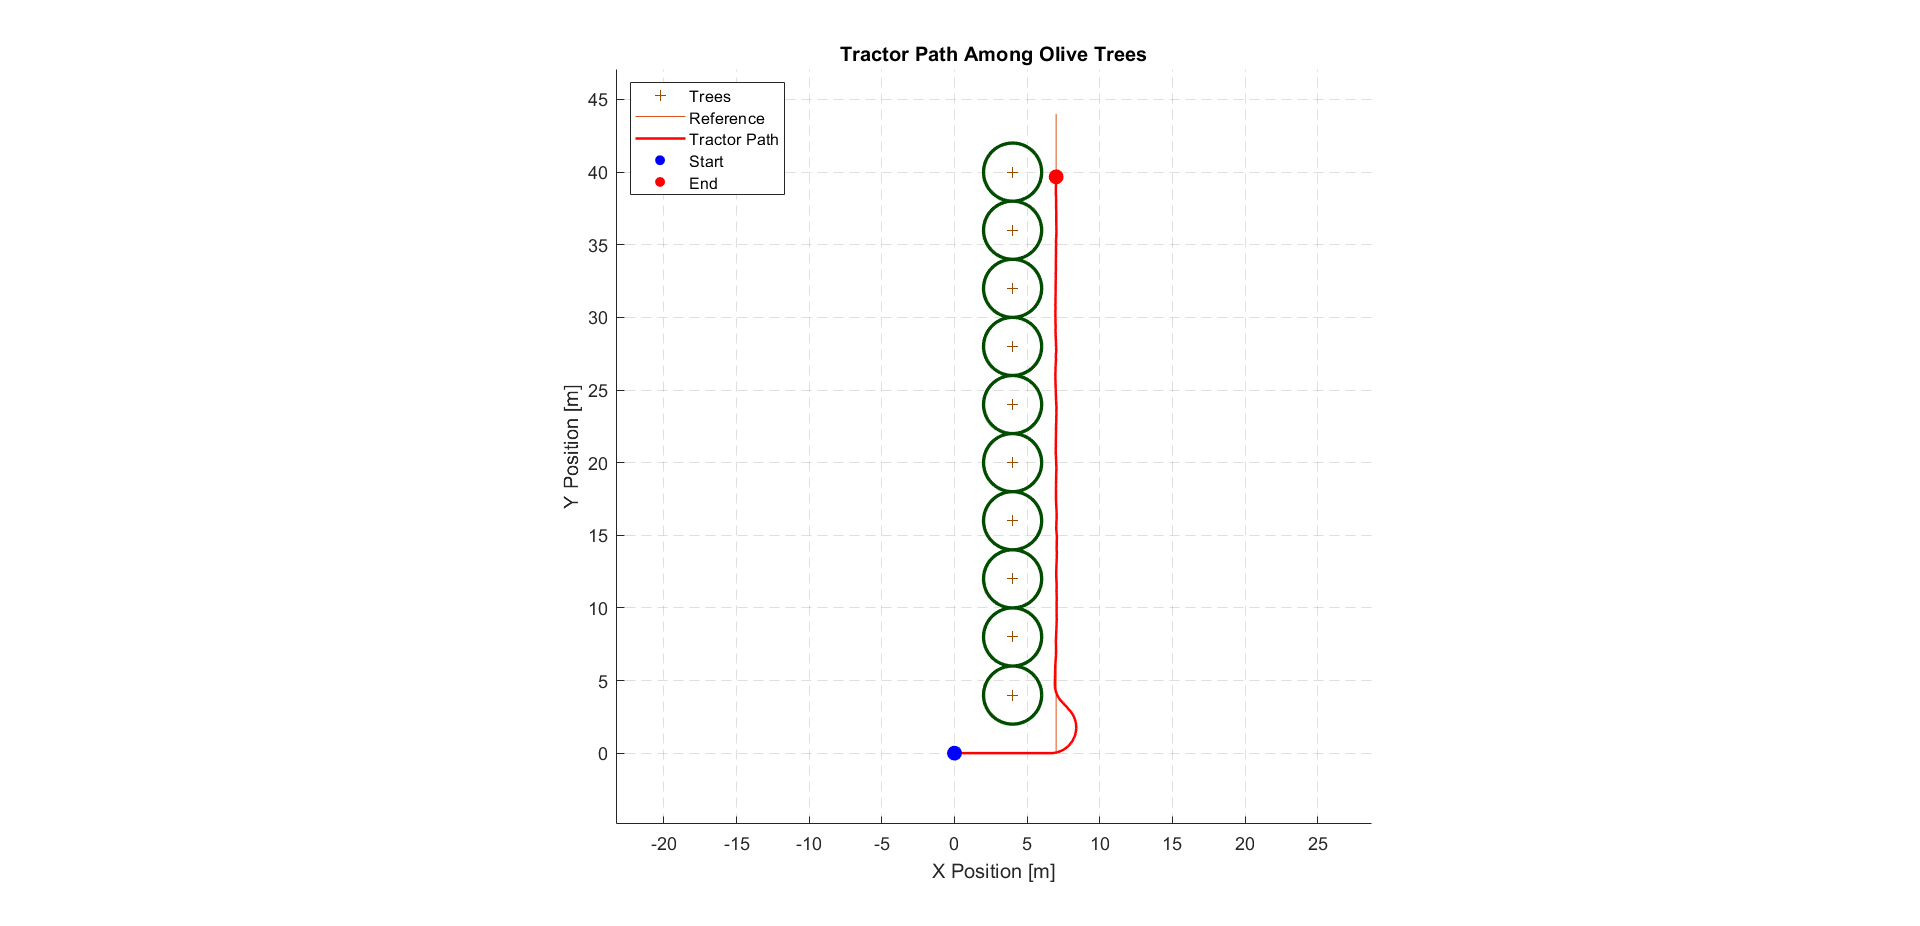
\includegraphics[width=\linewidth]{Imagens/ex2_results.png}
        \caption{Tractor path in the $x$--$y$ plane.}
        \label{fig:ex2_results}
    \end{figure}

    As shown in \cref{fig:ex2_results}, the controller successfully guides the tractor along the row while preserving the required safety distance.


    \subsection{Third Task}
    This task requires the integration of trajectory planning, speed control, and spraying actuation, taking into account the tractor dynamics, product consumption, and overall operational efficiency. The controller was implemented as a MATLAB function capable of coordinating all components of the autonomous spraying operation.

    In this scenario, the tractor velocity was assumed constant at \SI{40}{\kilo\meter\per\hour} explained why further along, and the same \gls{clf} controller used in previous tasks was employed. The agricultural environment consists of an intensive orchard layout, with \SI{6}{\meter} spacing between rows and \SI{4}{\meter} spacing between trees, each tree being modeled with a radius of \SI{2}{\meter}.

    Since the desired application rate is \SI{8}{\milli\liter} per tree, several simulation tests were performed to determine the nozzle aperture (\gls{valveOpening}) and the corresponding operating velocity required to achieve this target. The results showed that applying only \SI{8}{\milli\liter} per tree is not feasible under the given environmental conditions and hardware limitations, primarily due to the minimum continuous chemical application rate of the smallest available sprayer nozzle.

    Even with the smallest nozzle, which produces a spray radius of \SI{1.5}{\meter}, and operating at \SI{40}{\kilo\meter\per\hour}, approximately \SI{18}{\milli\liter} of product is applied to each tree. This outcome is illustrated in Figures~\cref{fig:tree_prod_inst} and \cref{fig:tree_prod_total}. The product delivered to a tree is computed as:

    \begin{equation}
        \text{product}_{\text{tree}} = \text{spray rate} \times \text{time step} \times 
        \left( \frac{\text{intersect area}}{\text{total spray area}} \right),
    \end{equation}

    where the spray rate varies linearly from \SI{9}{\liter\per\minute} at the minimum nozzle range up to \SI{14.4}{\liter\per\minute} for the maximum range.

    \begin{figure}[H]
        \centering
        \begin{minipage}{0.48\linewidth}
            \centering
            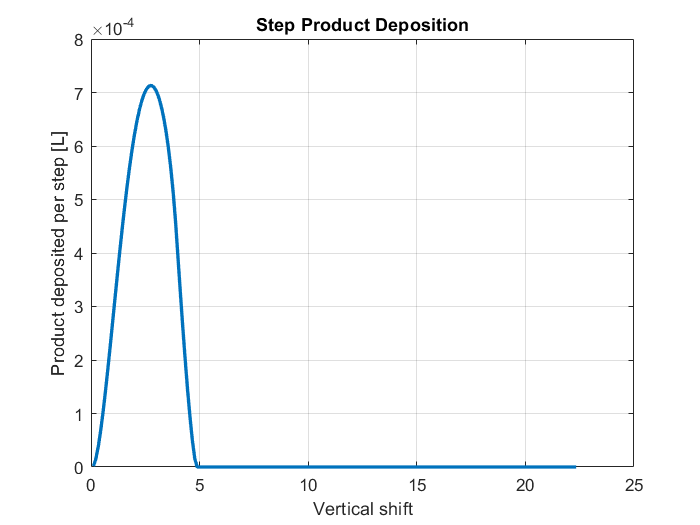
\includegraphics[width=\linewidth]{Imagens/tree_prod_inst.png}
            \caption{Instantaneous amount of product applied to a tree at each time step.}
            \label{fig:tree_prod_inst}
        \end{minipage}
        \hfill
        \begin{minipage}{0.48\linewidth}
            \centering
            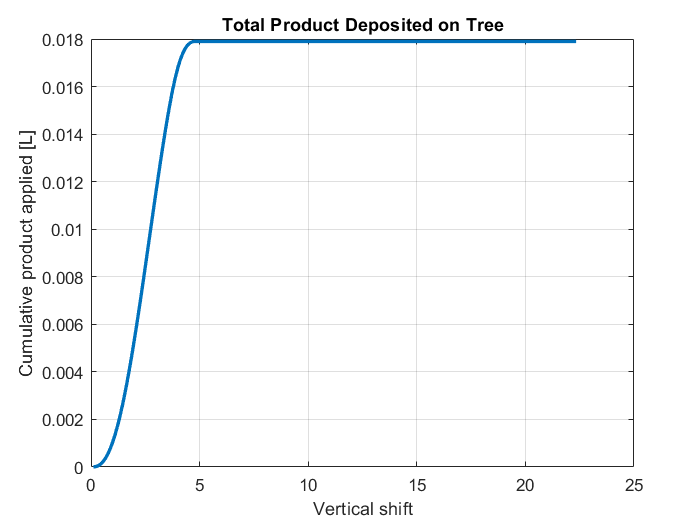
\includegraphics[width=\linewidth]{Imagens/tree_prod_total.png}
            \caption{Total amount of product applied to a tree.}
            \label{fig:tree_prod_total}
        \end{minipage}
    \end{figure}

    As it was already shown in \cref{sec:second_task} the system is cable of following the reference being only now added 2 extra refences after the begining/end of each row for the tractor to turn around and start spraying on the opossite direction on the next row. An example of this behavior is visible in~\cref{fig:ex3_results}.

    \begin{figure}[H]
        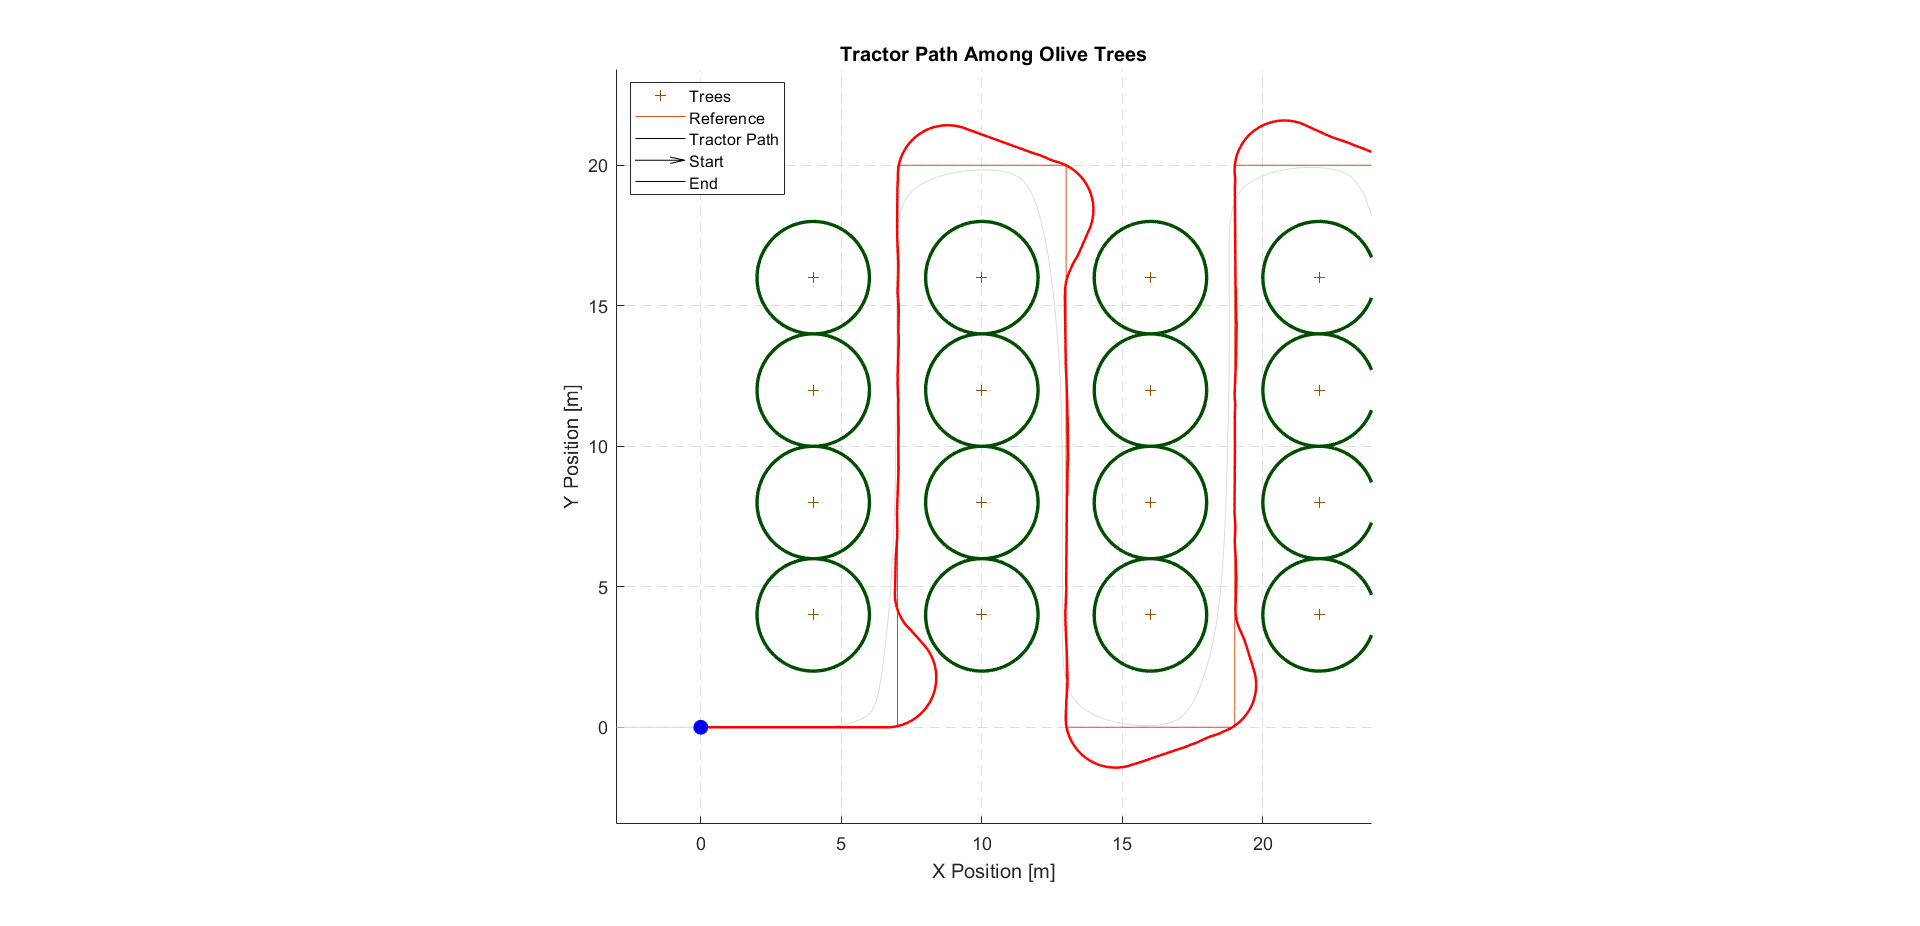
\includegraphics[width=\linewidth]{Imagens/ex3_results.png}
        \caption{Path from top view of the tractor}
        \label{fig:ex3_results}
    \end{figure}

    \end{document}